\chapter{Plotting}
\label{s:gui.plot}

One of the GUI's strong suits is the ability to view an manipulate plots using matplotlib.
Existing plots can be viewed and edited, and new templates can be defined on the fly.

Note: the GUI does support classic PG/PLplots, but it is recommended to use matplotlib as the plotting engine due to the extra fatures it offers.

%-----------------------------------------------------------------
\section{Viewing Plots}
\label{s:gui.plot.view}

\begin{figure}
\centering
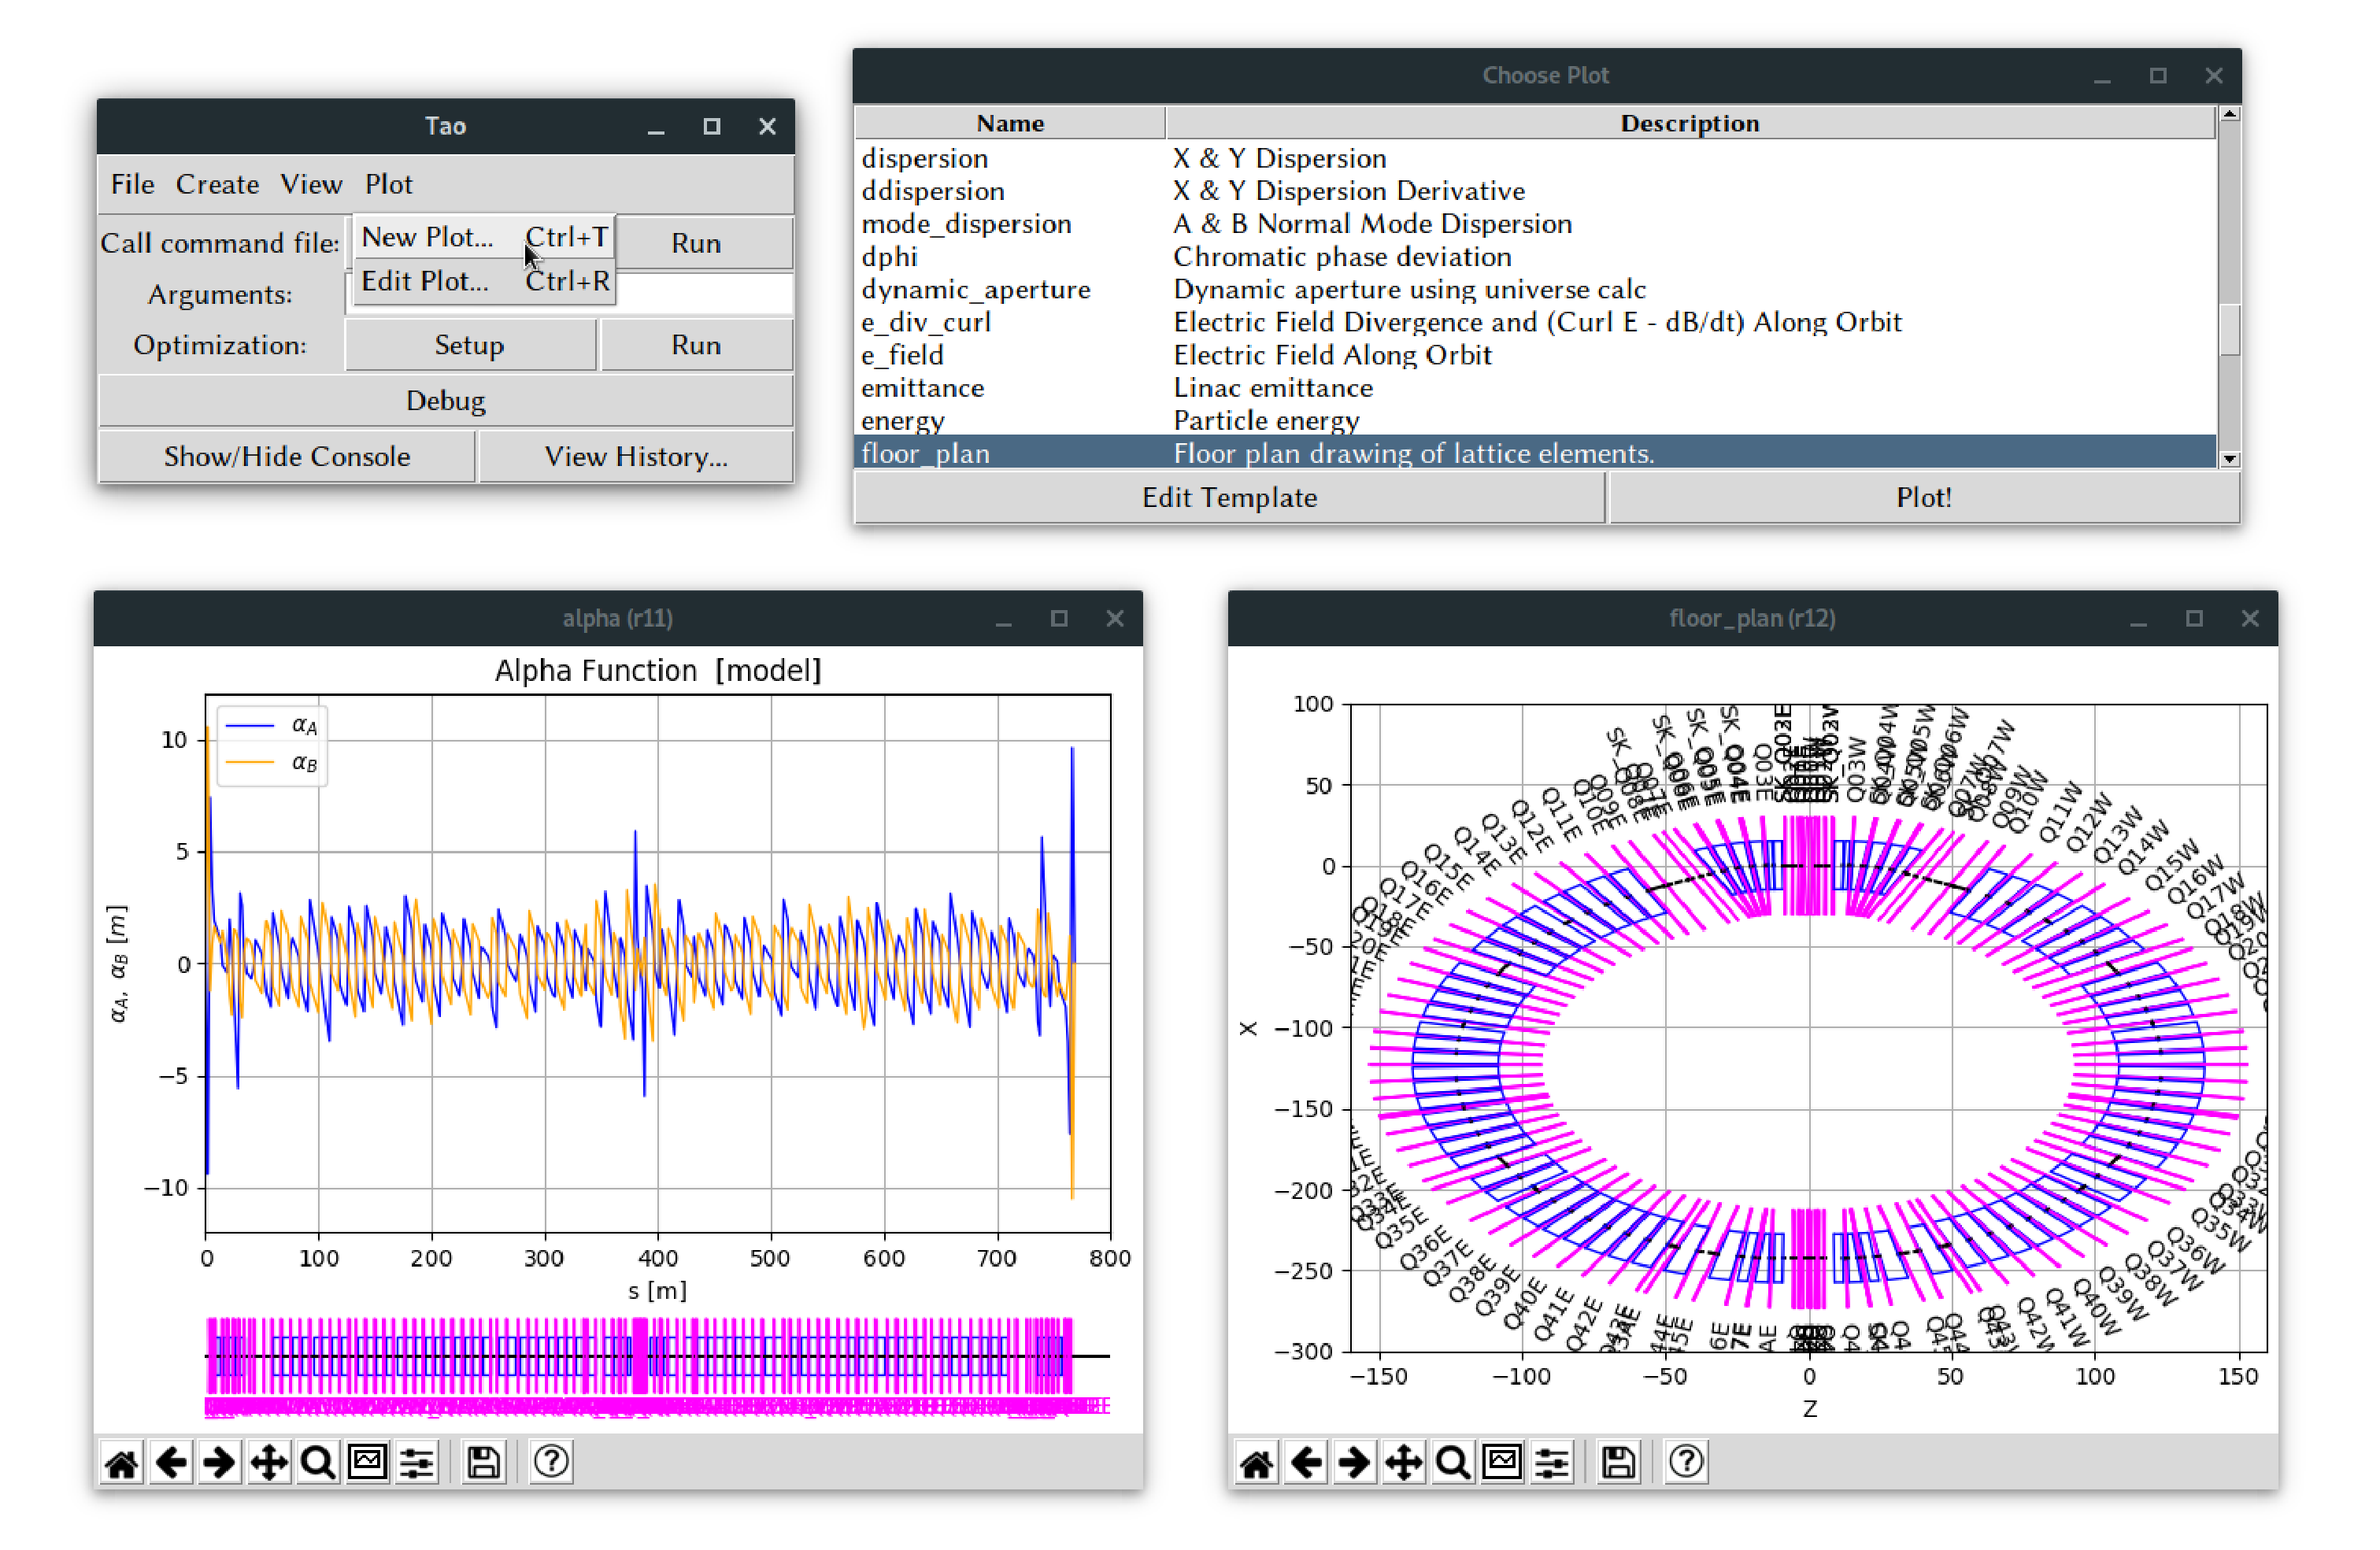
\includegraphics[width=12cm]{figures/view_plot.pdf}
\caption[Viewing plots with the GUI.]{Viewing plots with the GUI.
Top left: accessing the plot template list from the root window.
Top right: the plot template window.
Bottom left: a plot of the alpha function with the lat_layout shown below.
Bottom right: the floor_plan plot.}
\label{fig:gui.plot.view}
\end{figure}

Figure \ref{fig:gui.plot.view} shows how to plot existing templates in the GUI.
The plot template window lists all of the currently defined plot templates as well as their descriptions.
A template can be plotted either by double clicking on it, or by selecting it and then clicking the "Plot" button.
This will open a window displaying the selected plot (see Section \ref{s:gui.plot.interaction} for more information).
The user can also edit an existing template by selecting it in the tempalte window and clicking "Edit Template".

%-----------------------------------------------------------------
\section{Interacting with Plots}
\label{s:gui.plot.interaction}
Interacting with plots in the GUI is primarily done using the toolbar along the bottom of the plotting window.

Starting from the left, the home button returns the graph to the starting view. The back button returns to the previous view of the graph, working as an undo button. The forward button undoes the effects of the back button. All of these buttons also have keyboard shortcuts, 'h' or 'r' for home, 'c' or 'left arrow' for back, and 'v' or 'right arrow' for forward.

The pan/zoom button allows panning of the graph by holding a left click on the graph and dragging the mouse around. his mode also allows zooming of the graph by holding a right click on the graph and dragging the mouse around. These actions can be restricted to the horizontal axis by holding 'x' while dragging, or the vertical axis by holding 'y'. Holding 'control' while dragging the mouse will preserve aspect ratio. Clicking on the toolbar button again will get out of this mode.

The zoom to rectangle button allows a rectangle to be selected by holding a left click on the graph and dragging the mouse, which will then fill the graph window. Holding 'x' or 'y' while selecting a rectangle will only effect the horizontal or vertical axis respectively.

The save button allows the graph window to be saved as an image file. Using 'ctrl+s' has the same effect.

If any floor plan or lat layout is present, double clicking on an element will open a window to view or edit element parameters.

Floor plans contain a slider to scale the size of elements away from the element centerline. Clicking on the slider will adjust the width of the displayed elements.

%-----------------------------------------------------------------
\section{Plotting Initialization}
\label{s:gui.plot.init}

When operating the GUI in matplotlib mode, you can specify a list of template plots to plot in matplotlib as soon as tao starts.  These templates should be listed in a file called plot.gui.init, which should be in the same directory from which you launch the gui.

plot.gui.init should have one template listed per line and absolutely nothing else on the line.  The templates listed in plot.gui.init are checked against the list of templates that tao can plot, and if a template is not recognized it is simply ignored.

